\documentclass[sigplan,screen]{acmart}
\usepackage{todonotes}

\newcommand{\TODO}[1]{\todo[inline]{#1}}

\setcopyright{acmcopyright}
\copyrightyear{2022}
\acmYear{2022}
\acmDOI{XXXXXXX.XXXXXXX}

\acmConference[Conference acronym 'XX]{Make sure to enter the correct
  conference title from your rights confirmation emai}{June 03--05,
  2018}{Woodstock, NY}
%\acmBooktitle{Woodstock '18: ACM Symposium on Neural Gaze Detection,
%  June 03--05, 2018, Woodstock, NY} 
\acmPrice{15.00}
\acmISBN{978-1-4503-XXXX-X/18/06}
%%\acmSubmissionID{123-A56-BU3}
%%\citestyle{acmauthoryear}

\begin{document}

\title{MLCommons Earthquake Science Benchmark}

\author{Thomas Butler}
\email{trovato@corporation.com}
\author{G.K.M. Tobin}
\email{webmaster@marysville-ohio.com}
\affiliation{%
  \institution{University of Virginia}
  \streetaddress{TBD}
  \city{Charlotsville, VA}
  \country{USA}}

\author{Robert Knuuti}
\affiliation{%
  \institution{University of Virginia}
  \streetaddress{TBD}
  \city{Charoletteville}
  \country{USA}}
\email{uqq5zz@virginia.edu}

\author{Jake Kolessar}
\affiliation{%
  \institution{University of Virginia}
  \streetaddress{TBD}
  \city{Charoletteville}
  \country{United States}}
\email{jakekolessar@gmail.com}

\author{Geoffrey C. Fox}
\affiliation{%
  \institution{University of Virginia}
  \streetaddress{TBD}
  \city{Charlotsville, VA}
  \country{USA}}
\email{gcfexchange@gmail.com}

\author{Gregor von Laszewski}
\orcid{0000-0001-9558-179X}
\affiliation{%
  \institution{University of Virginia}
  \streetaddress{TBD}
  \city{Charlotsville, VA}
  \country{USA}}
\email{laszewski@gmail.com}


\renewcommand{\shortauthors}{Buttler, Knuuti, Kolesar, Fox, von Laszewski}

\begin{abstract}
TBD
\end{abstract}

%% see http://dl.acm.org/ccs.cfm.
\begin{CCSXML}
<ccs2012>
 <concept>
  <concept_id>10010520.10010553.10010562</concept_id>
  <concept_desc>Computer systems organization~Embedded systems</concept_desc>
  <concept_significance>500</concept_significance>
 </concept>
 <concept>
  <concept_id>10010520.10010575.10010755</concept_id>
  <concept_desc>Computer systems organization~Redundancy</concept_desc>
  <concept_significance>300</concept_significance>
 </concept>
 <concept>
  <concept_id>10010520.10010553.10010554</concept_id>
  <concept_desc>Computer systems organization~Robotics</concept_desc>
  <concept_significance>100</concept_significance>
 </concept>
 <concept>
  <concept_id>10003033.10003083.10003095</concept_id>
  <concept_desc>Networks~Network reliability</concept_desc>
  <concept_significance>100</concept_significance>
 </concept>
</ccs2012>
\end{CCSXML}

\ccsdesc[500]{Computer systems organization~Embedded systems}
\ccsdesc[300]{Computer systems organization~Redundancy}
\ccsdesc{Computer systems organization~Robotics}
\ccsdesc[100]{Networks~Network reliability}

%%
%% Keywords. The author(s) should pick words that accurately describe
%% the work being presented. Separate the keywords with commas.
\keywords{MLCommons, Science AI Benchmark, Earthquake, Deep Learning}

\maketitle

\section{Introduction}

\subsection{MLCommons}

\subsection{Earthquake prediction}

Things to do: 
\begin{itemize}
    %\item add presentation as cite,
    \item Review IEEE Presentation \cite{fox2022aiforscience}
    \item Review MLCommons \cite{www-mlcommons} 
    \item Use jabref \cite{www-jabrefg-org} for citation management
    \item Review Fox paper \cite{fox2021earthquake}
    \item Frequently check github \cite{www-mlcommons-eathquake}
    \item Read up on TFT \cite{www-onnen2021}
    \item Become familiar with the Attention Paper \cite{vaswani2017attention}
    \item Learn how to selfdeploy jupyterlab \cite{www-jupyterlab}
    \TODO{Is this the same as jupytext?}
    
    \item Begin to learn about papermill \cite{www-papermill} \TODO{Rivanna's core configurations might be a bit limited on this front.  They do provide multiple versions of software (such as py2.7 and py3.8), but we may need to get permission to do something in userspace if we need to be very specific on a version of python.  Do we want to look into using tox, conda, or leave this up to the container ecosystem to solve?}
    \TODO{Gregor: add how to use conda and modules to switch python versions}
    \item virtualenv on rivanna for a particular python version.
    \item depends on Tensorflow
    \TODO{Below this line are objectives or targets to take the current modeling solution and mature it for other platforms / ecosystems.  Rivanna uses Lua's lmod ecosystem for jailing a process, and anaconda uses solved environments for dependencies that extend beyond just python modules.}
    \item Familiarize yourself with Rivanna's modules \cite{www-modules}  and conda \cite{www-conda} environments.
    \item pytorch \cite{www-pytorch}
    \TODO{There is interest in comparing pytorch and tensoflow}
    \item horovod \cite{www-horovod}
    \TODO{MLCommons project that can target a few platforms using a YAML contract.  Once we solve the target environment, we can likely target porting this way.}
    \TODO{Also, good news is Rivanna has a Singularity module  as an lmod (3.7.1), so we might be able to use that as a targeted runner without having to setup too much additional scaffolding.
    And if things work right, we could use the k8s module to do local deployments if we wanted to test out alternate execution paths. }
    \item mlcube \cite{www-mlcube} 
\end{itemize}

%\begin{figure}[h]
%  \centering
%  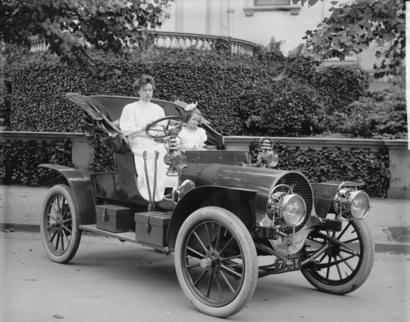
\includegraphics[width=\linewidth]{sample-franklin}
%  \caption{1907 Franklin Model D roadster. Photograph by Harris \&
%    Ewing, Inc. [Public domain], via Wikimedia
%    Commons. (\url{https://goo.gl/VLCRBB}).}
%  \Description{A woman and a girl in white dresses sit in an open car.}
% \end{figure}

\section{Benchmarks}

\subsection{Hardware}

\subsection{University of Virginia Rivanna}
\label{id:uva} 

UVA, Rivanna, A100, RTX3090, others may not have enough memory. 
\TODO{description of Rivanna on web page is not accurate.}

\subsection{Rutherfordlab ???}
\label{id:ral} 

Rutherfordlab (RAL)

\subsection{Summit}
\label{id:ornl} 

Oak Ridge National Labratory (ORNL), Summit

\subsection{NERSC ???}
\label{id:nersc} 

National Energy Research Scientific Computing Center (NERSC), ...

\subsection{Aurora}
\label{id:anl} 

Argonne National Laboratory (ANL), ...

\subsection{SDSC}
\label{id:sdcs} 

San Diego Super Computing Center, ...


\subsection {Nvidia DGX Workstation}

\label{id:dgx} DGX Fox \cite{www-dgx-station-a100}

\begin{table*}[htb]
    \caption{Overview of compute resources.}
    \label{tab:my_label}
    \centering
    \begin{tabular}{|r|l|l|r|l|l|l|}
        \hline
        Section & Organization & Machine  & Processors & GPUs & GPU Type  & Commissioned \\ 
        \hline
        \hline
         \ref{id:uva}   & UVA       & Rivanna   &            &      &           & \\
         \ref{id:ral}   & RAL       &           &            &      &           & \\
         \ref{id:ornl}  & ORNL      &  Summit   &            &      &           & \\
         \ref{id:nersc} & NERSC     &           &            &      &           & \\
         \ref{id:anl}   & ANL       &           &            &      &           & \\
         \ref{id:sdsc}  & SDSC      &           &            &      &           & \\
         \ref{id:dgx}   & DGX Staion A100   &           & 1          &  AMD EPYC 7742 64-Core Processor   & A100 80GB  & Fox will know\\
         \hline
    \end{tabular}
\end{table*}


\begin{acks}
\TODO{Geoffrey: please add acknowledgement for funding, other acks}
\end{acks}

\bibliographystyle{ACM-Reference-Format}
\bibliography{references,sample-base}

\clearpage

\appendix

\section{Manuals Developed}

The following manuals have been developed by the team:

\begin{itemize}
    \item Introduction to Python \cite{las-intro-python}
\end{itemize}

\section{Todo}

\listoftodos

Robert: I am moving the rough notes into our github repo and made a 

\begin{itemize}
\item \href{https://github.com/cybertraining-dsc/capstone-eartquake/blob/main/TODO.md}{TODO.md} 
\end{itemize}

file that we can use to build a simple list of things we want to do.  I'll leave them in the overleaf for now, but I feel like that's not a good home for that type of information given that it's mean to be the paper to submit on the subject.

\TODO{Not sure if we want to talk about building tasks / kanban boards to track the different parts of work we'll be doing each week.  Additionally, it might be good to decide on some core roles to make sure things don't fall through the cracks (roles like recorder, scheduler, reviewer, et al...); the non-technical stuff for now, and then we can get into the more specific things once we pass the initial knowledge rampup}

\end{document}
\endinput
%%
%% End of file `sample-sigplan.tex'.
